
\section{Desarrollo visual y flujo completo}
La distribución adapta los wireframes de referencia de la guía sin utilizar sus importes ilustrativos como reglas. Las capturas se copiaron sin modificar sus píxeles desde las evidencias del commit publicado. El manifiesto de procedencia incluye URL y SHA256. No se utilizan imágenes decorativas dentro de la aplicación.

Los ejecutores crean una base aislada autentican los perfiles y usan formularios reales. Las operaciones se realizan mediante los servicios y comandos del sistema y las vistas se refrescan antes de generar la imagen con DrawToBitmap. No se afirma que todo el recorrido se haya realizado mediante clics manuales.
Algunas figuras muestran recortes de las zonas operativas para evitar espacios vacíos y facilitar la lectura Los PNG originales permanecen completos y sus hashes no cambian

\noindent\begin{minipage}{\linewidth}\subsection{Acceso local}
La ventana recibe usuario y contraseña y delega en Autenticacion. El servicio verifica el hash y establece la sesión. Los permisos vuelven a comprobarse en los casos de uso.

\begin{center}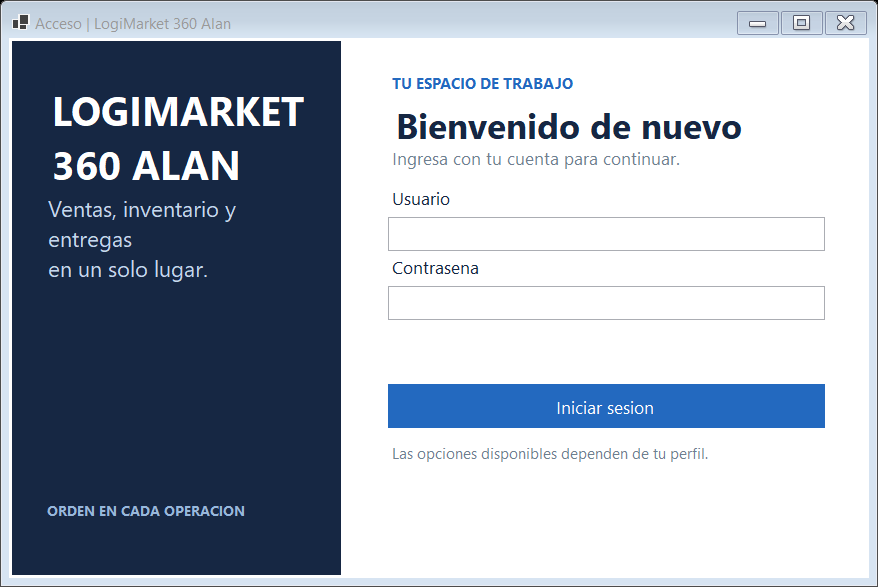
\includegraphics[width=\linewidth,height=9.5cm,keepaspectratio]{imagenes/acceso.png}
\captionof{figure}{Acceso local}\label{fig:acceso}\end{center}
\end{minipage}\par\bigskip
\noindent\begin{minipage}{\linewidth}\subsection{Navegación según el rol}
Los perfiles muestran solamente sus apartados VENTAS opera ventas BODEGA inventario y despacho y CONSULTA dispone de lectura Los servicios comprueban también los permisos

\begin{center}
\begin{minipage}[t]{0.31\linewidth}\centering\textbf{VENTAS}\\[4pt]
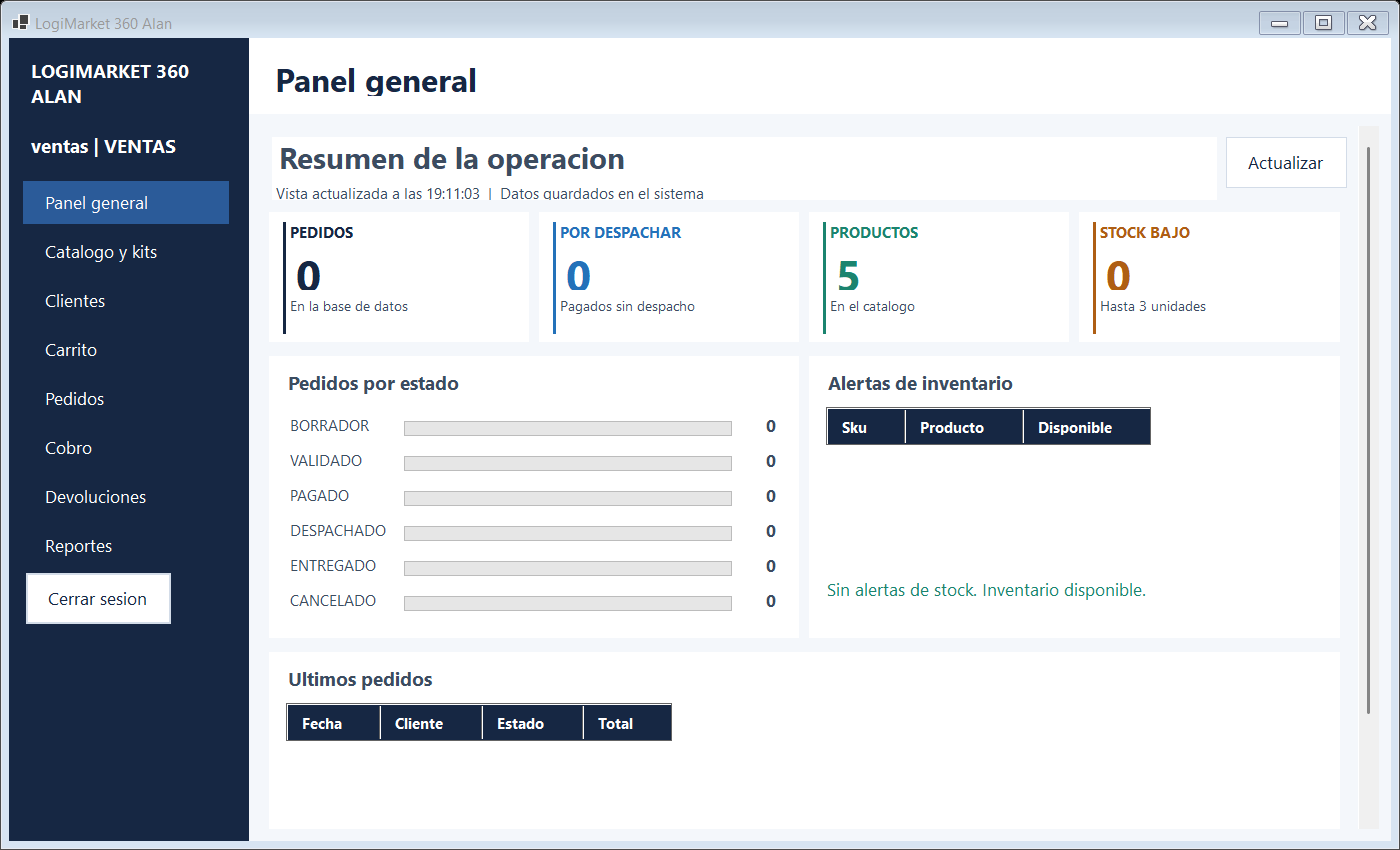
\includegraphics[width=\linewidth,height=15cm,keepaspectratio,trim=0bp 0bp 690.06bp 0bp,clip]{imagenes/ventas.png}
\end{minipage}\hfill
\begin{minipage}[t]{0.31\linewidth}\centering\textbf{BODEGA}\\[4pt]
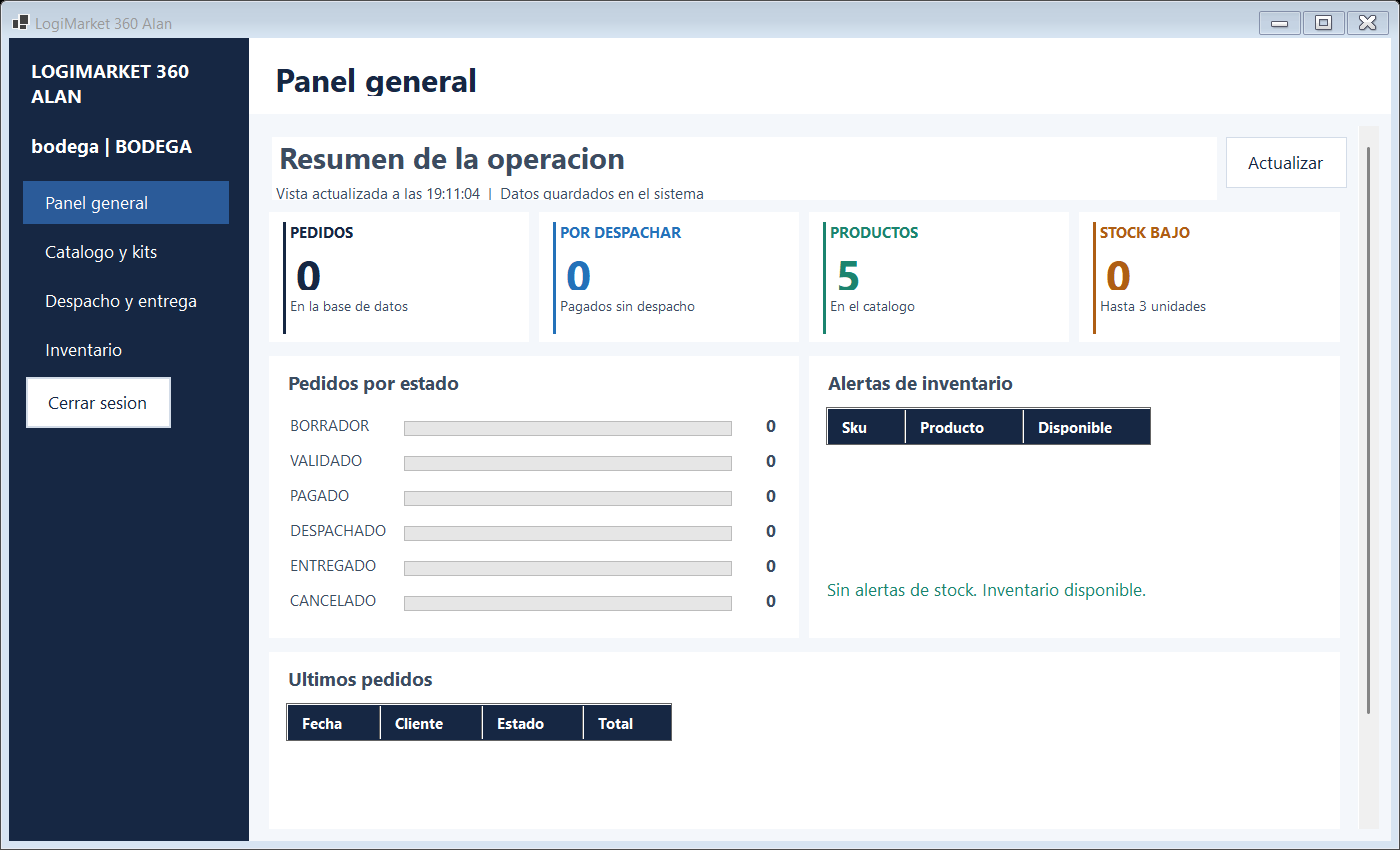
\includegraphics[width=\linewidth,height=15cm,keepaspectratio,trim=0bp 0bp 690.06bp 0bp,clip]{imagenes/bodega.png}
\end{minipage}\hfill
\begin{minipage}[t]{0.31\linewidth}\centering\textbf{CONSULTA}\\[4pt]
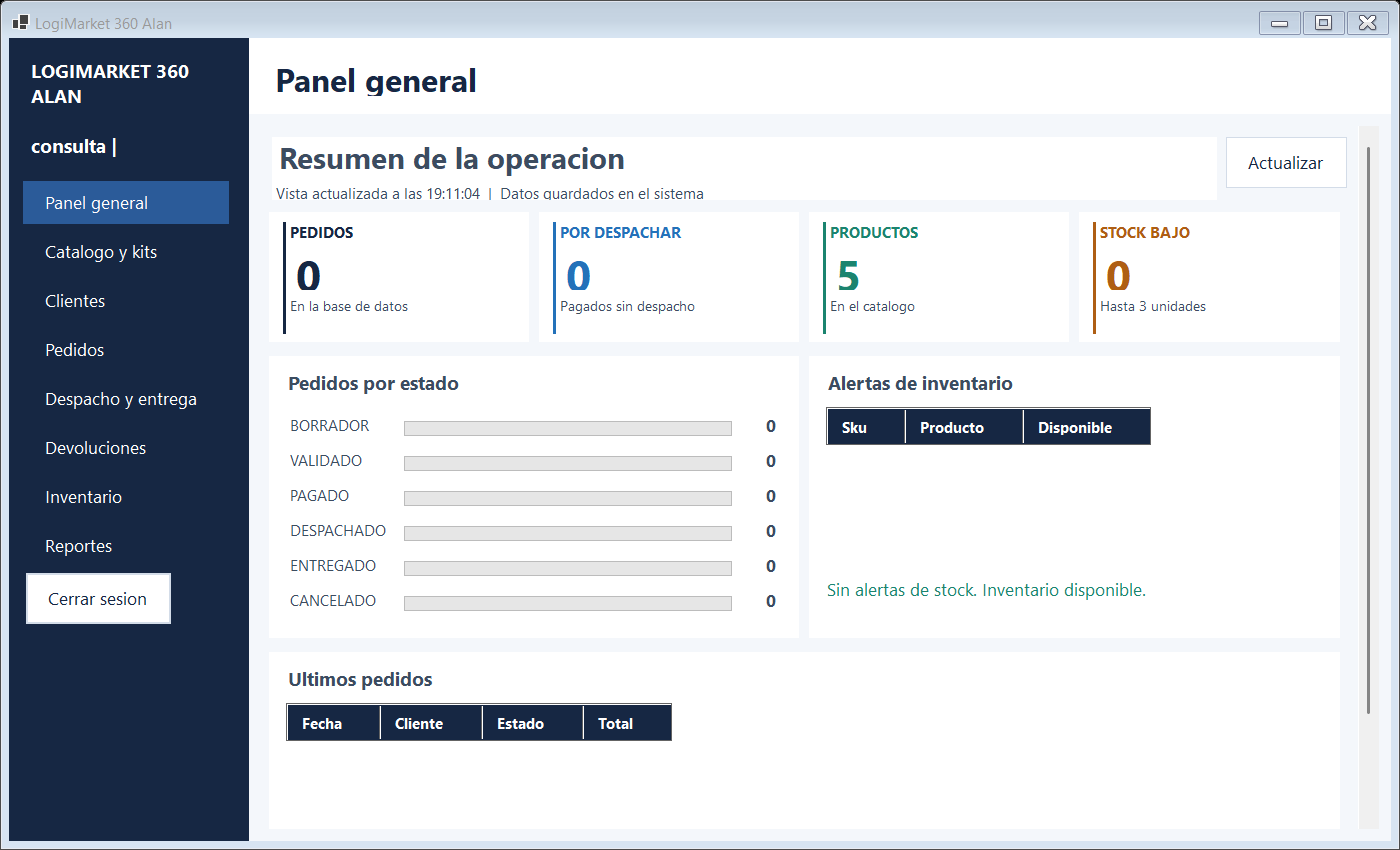
\includegraphics[width=\linewidth,height=15cm,keepaspectratio,trim=0bp 0bp 690.06bp 0bp,clip]{imagenes/consulta.png}
\end{minipage}\hfill
\captionof{figure}{Recortes de los menús reales de los tres perfiles operativos}\label{fig:roles}\end{center}\end{minipage}\par\bigskip
\noindent\begin{minipage}{\linewidth}\subsection{Catálogo con productos y kits de control}
El listado muestra los cinco productos y dos kits. Se verifican precios 50.00 y 60.00 y peso 1.00 kg para teletrabajo. El kit calcula disponibilidad desde sus hojas físicas.

\begin{center}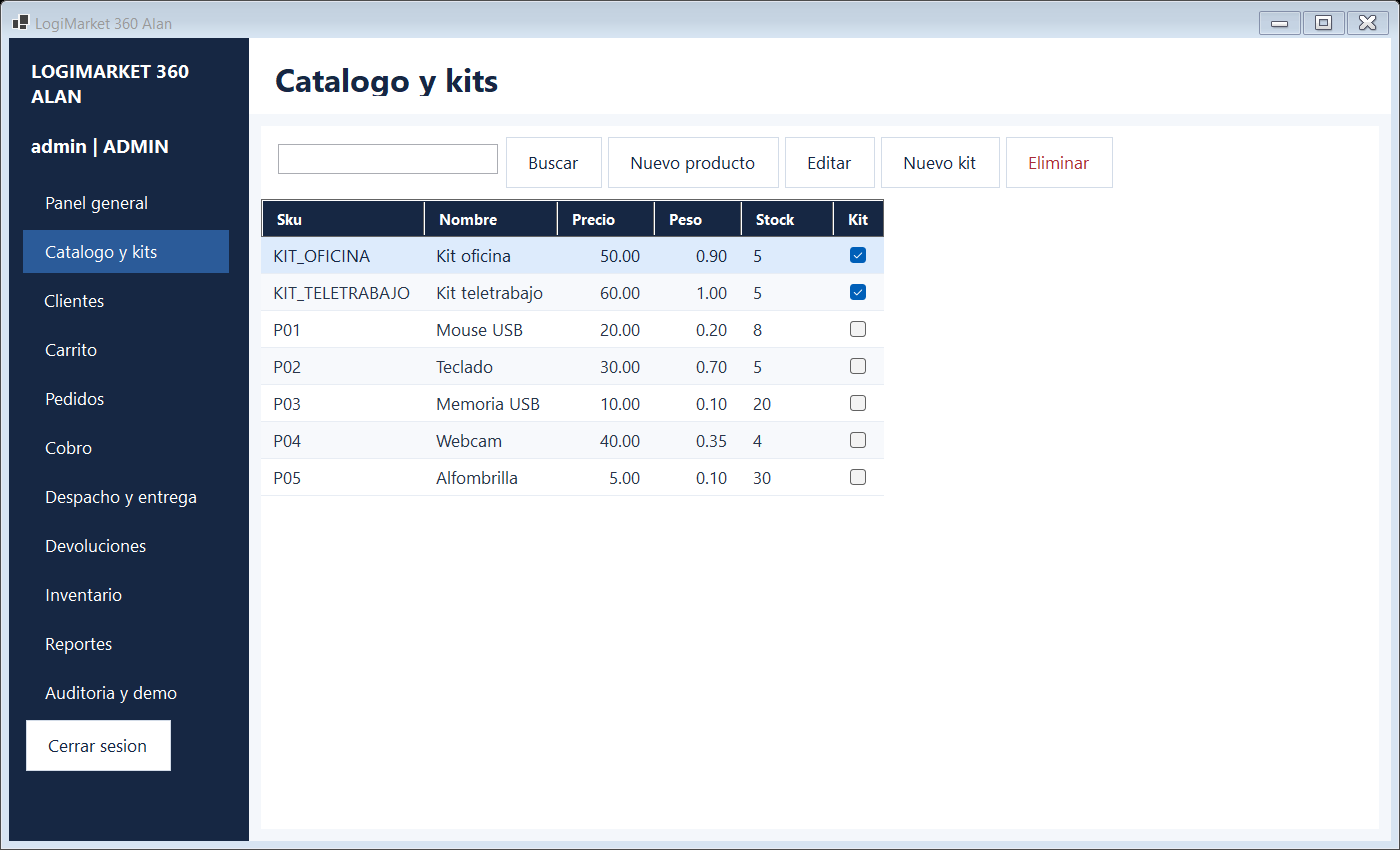
\includegraphics[width=\linewidth,height=9.5cm,keepaspectratio,trim=148.81bp 180.02bp 0.00bp 0bp,clip]{imagenes/vista-Catalogo-y-kits.png}
\captionof{figure}{Catálogo con productos y kits de control}\label{fig:catalogo}\end{center}
\end{minipage}\par\bigskip
\noindent\begin{minipage}{\linewidth}\subsection{Clientes iniciales del caso académico}
Ana es VIP y Luis y Carmen son NORMAL La promoción mayorista no requiere una categoría persistida adicional depende de la cantidad física comprada.

\begin{center}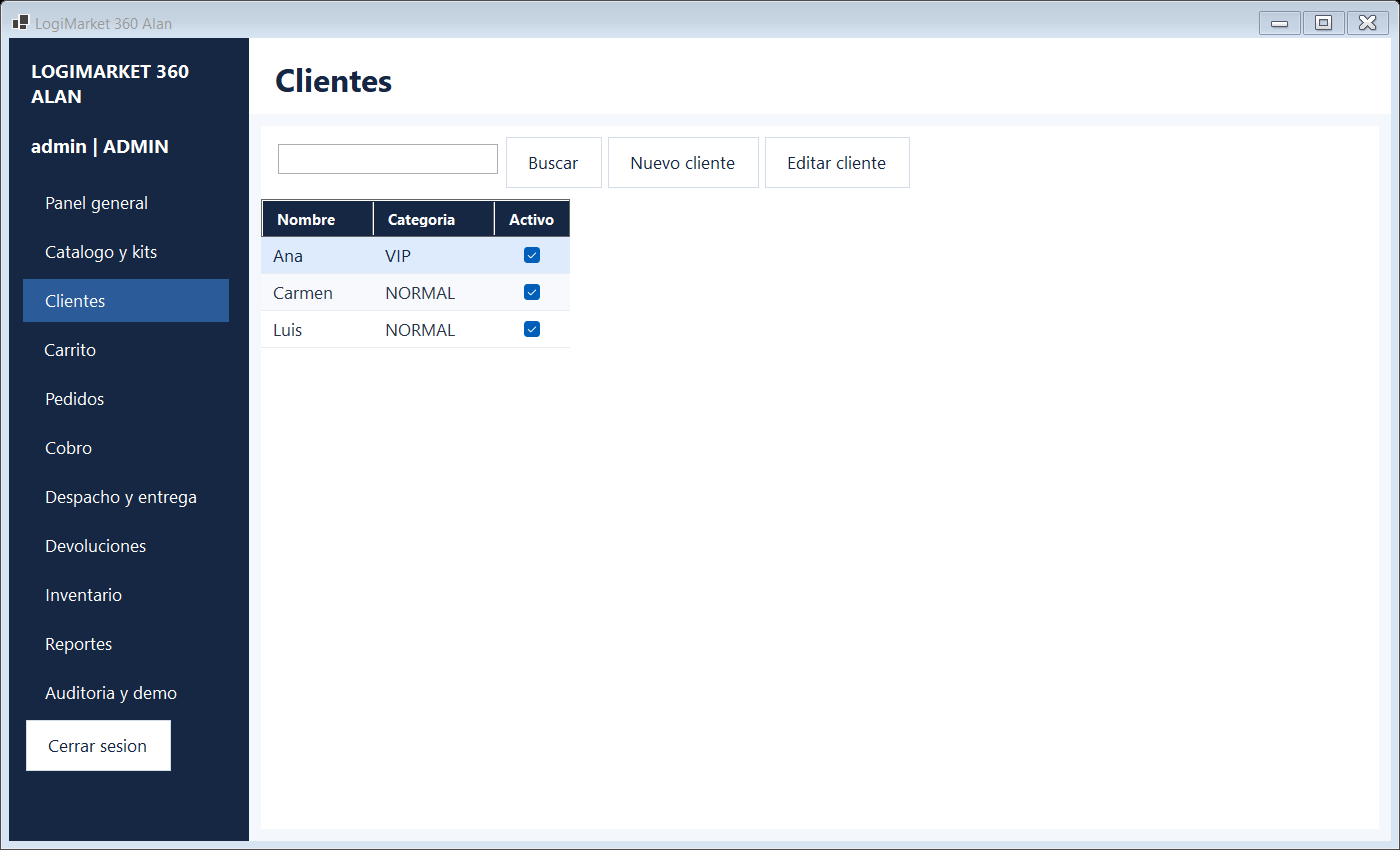
\includegraphics[width=\linewidth,height=9.5cm,keepaspectratio,trim=148.81bp 291.03bp 0.00bp 0bp,clip]{imagenes/vista-Clientes.png}
\captionof{figure}{Clientes iniciales del caso académico}\label{fig:clientes}\end{center}
\end{minipage}\par\bigskip
\noindent\begin{minipage}{\linewidth}\subsection{Carrito con acciones de borrador}
El formulario permite agregar cambiar quitar líneas guardar y deshacer o rehacer. La captura corresponde al estado inicial vacío y no se presenta como prueba de una venta ya guardada.

\begin{center}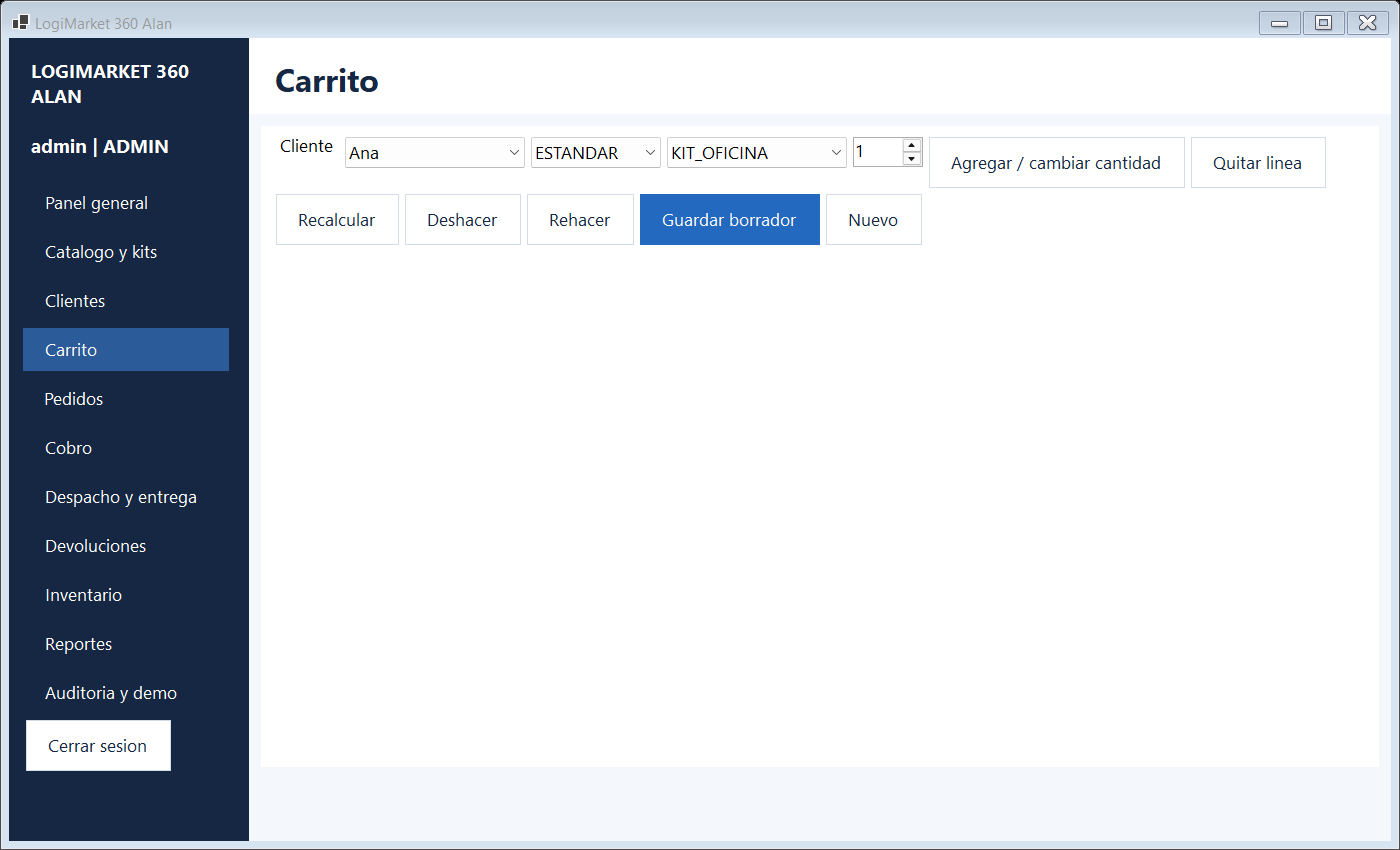
\includegraphics[width=\linewidth,height=9.5cm,keepaspectratio,trim=148.81bp 291.03bp 0.00bp 0bp,clip]{imagenes/vista-Carrito.png}
\captionof{figure}{Carrito con acciones de borrador}\label{fig:carrito}\end{center}
\end{minipage}\par\bigskip
\noindent\begin{minipage}{\linewidth}\subsection{Consulta de pedidos y acciones del perfil administrador}
Los filtros e historial permiten seguir el ciclo En esta captura inicial todavía no hay filas. Las evidencias posteriores muestran el pedido real procesado.

\begin{center}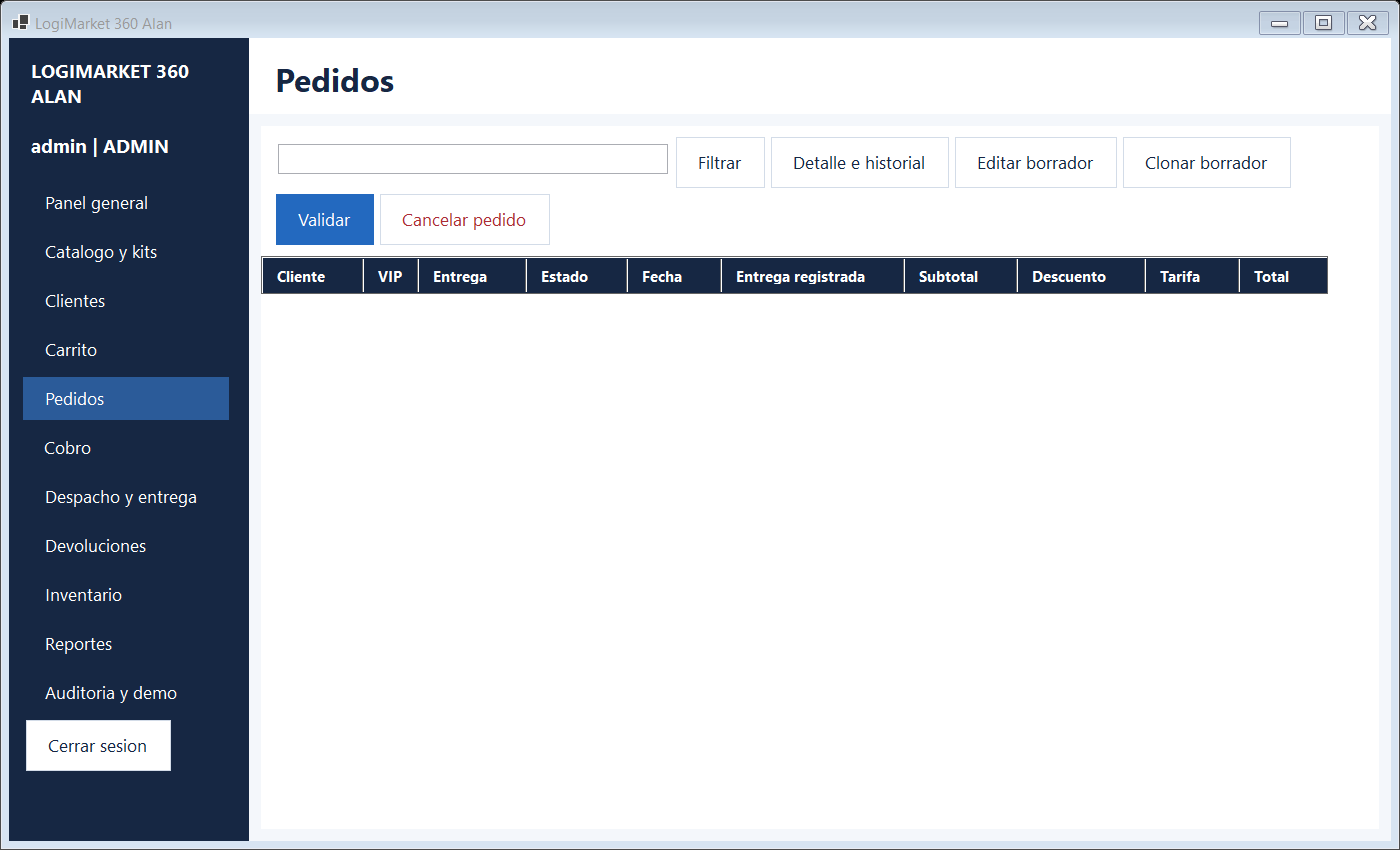
\includegraphics[width=\linewidth,height=9.5cm,keepaspectratio,trim=148.81bp 291.03bp 0.00bp 0bp,clip]{imagenes/vista-Pedidos.png}
\captionof{figure}{Consulta de pedidos y acciones del perfil administrador}\label{fig:pedidos}\end{center}
\end{minipage}\par\bigskip
\noindent\begin{minipage}{\linewidth}\subsection{Pedido de Ana pagado por USD 59.00}
La confirmación dejó subtotal 60.00 descuento 6.00 tarifa 5.00 y total 59.00. El mismo comando puede invocarse desde la pantalla y el ejecutor de prueba.

\begin{center}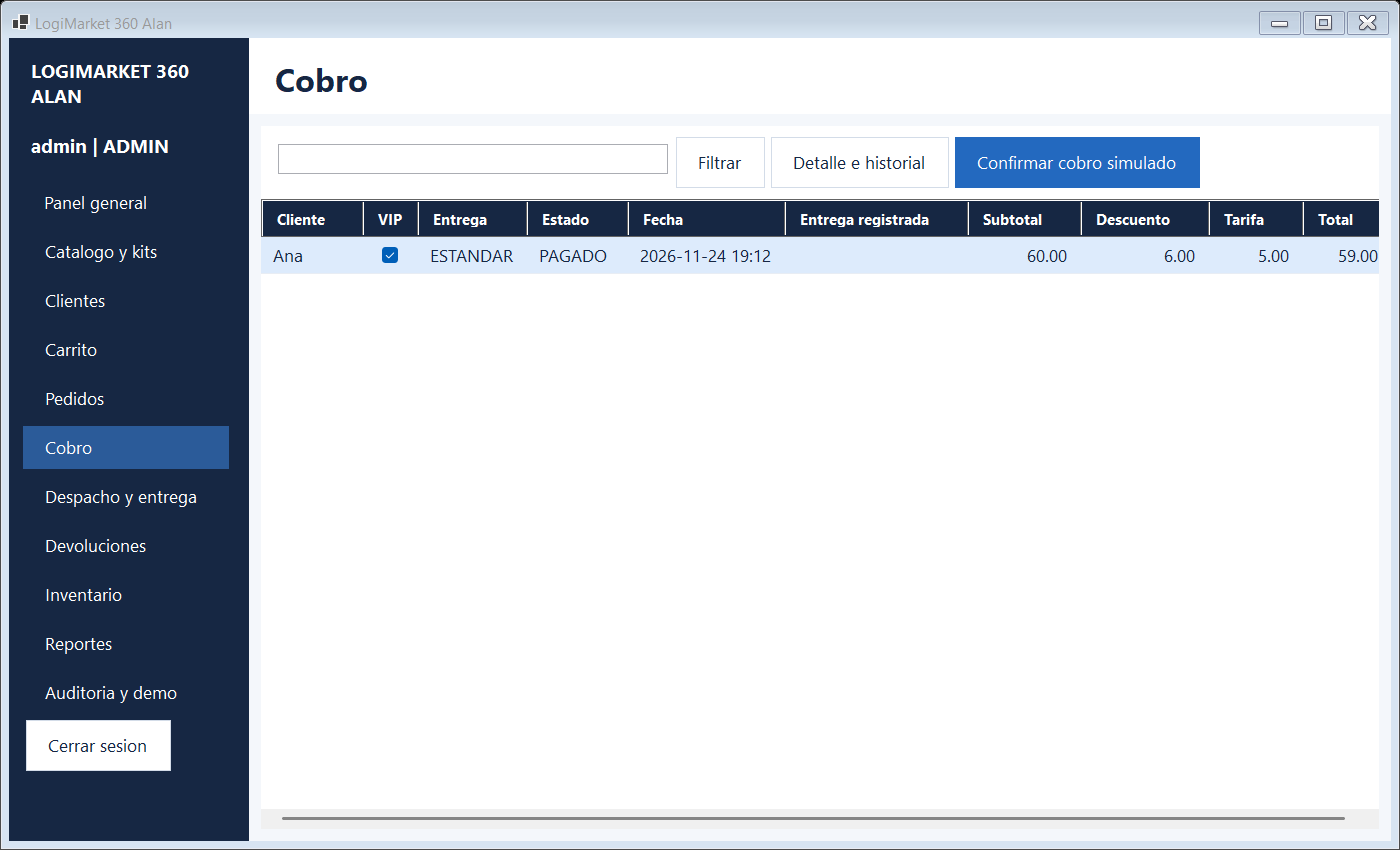
\includegraphics[width=\linewidth,height=9.5cm,keepaspectratio,trim=148.81bp 240.02bp 0.00bp 0bp,clip]{imagenes/flujo-01-cobro.png}
\captionof{figure}{Pedido de Ana pagado por USD 59.00}\label{fig:cobro}\end{center}
\end{minipage}\par\bigskip
\noindent\begin{minipage}{\linewidth}\subsection{Existencias y movimientos después del cobro}
P01 queda en 7 P02 en 4 y P03 en 19. Cada salida conserva motivo y referencia. El despacho no vuelve a descontar esas existencias.

\begin{center}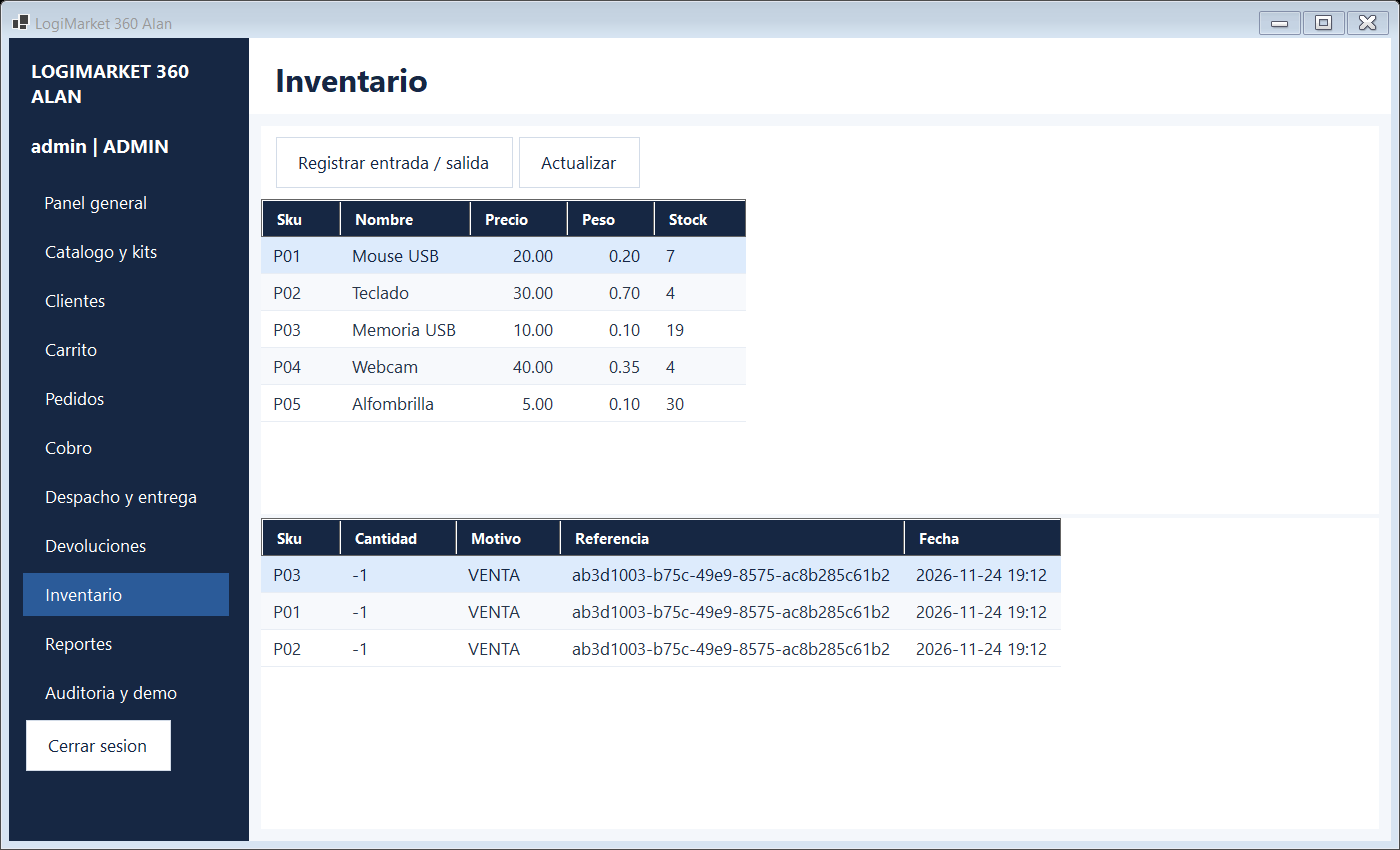
\includegraphics[width=\linewidth,height=9.5cm,keepaspectratio,trim=148.81bp 0.00bp 0.00bp 0bp,clip]{imagenes/flujo-02-stock.png}
\captionof{figure}{Existencias y movimientos después del cobro}\label{fig:stock}\end{center}
\end{minipage}\par\bigskip
\noindent\begin{minipage}{\linewidth}\subsection{Pedido entregado y guía logística}
Después del pago se registraron despacho y entrega. Una cancelación posterior fue rechazada conservando el estado ENTREGADO.

\begin{center}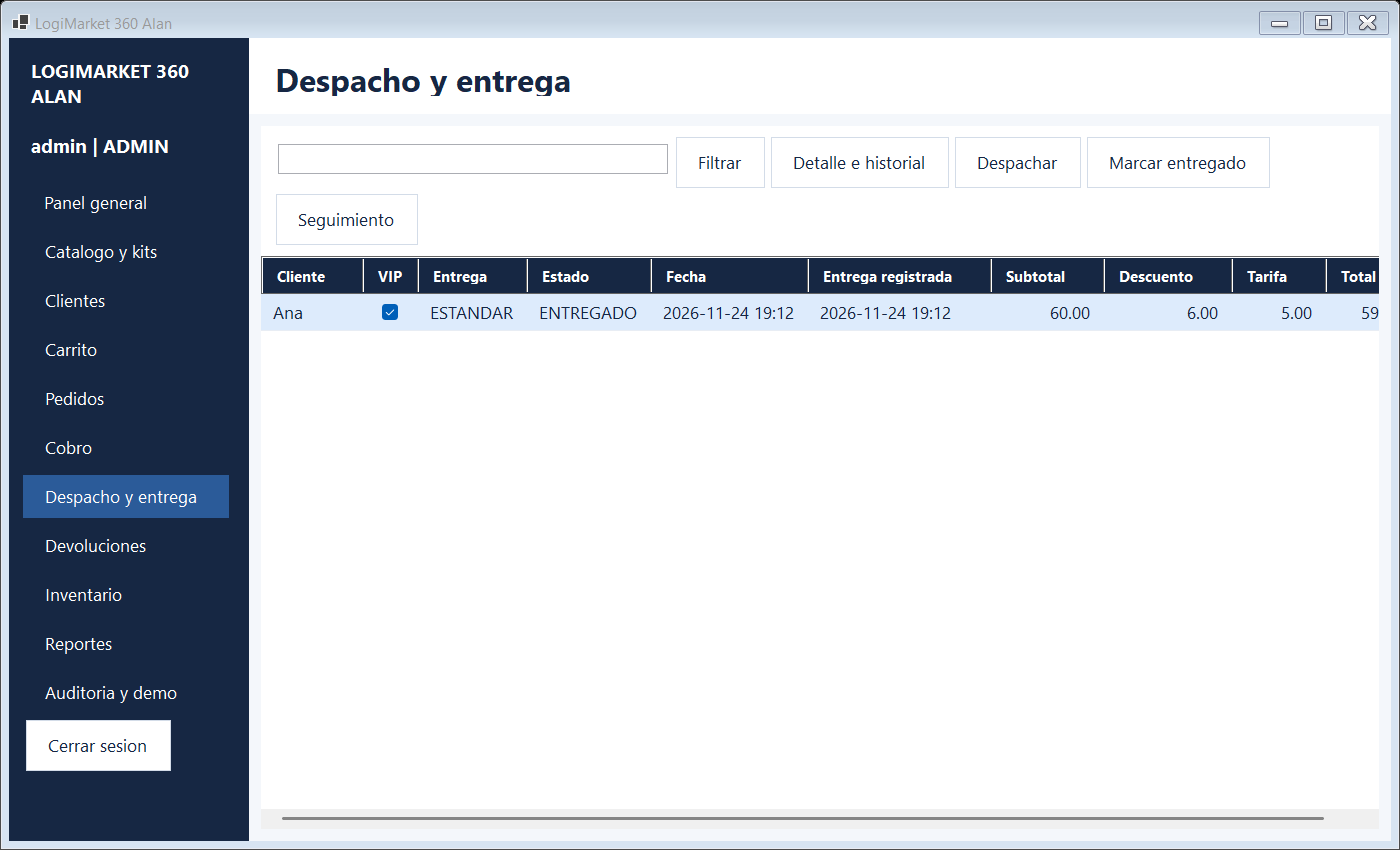
\includegraphics[width=\linewidth,height=9.5cm,keepaspectratio,trim=148.81bp 240.02bp 0.00bp 0bp,clip]{imagenes/flujo-03-entregado.png}
\captionof{figure}{Pedido entregado y guía logística}\label{fig:entregado}\end{center}
\end{minipage}\par\bigskip
\noindent\begin{minipage}{\linewidth}\subsection{Inventario después de la devolución aceptada}
La devolución por DEFECTO reembolsó 54.00 sin envío y reintegró P01 a 8 P02 a 5 y P03 a 20. El segundo intento no puede duplicar el reintegro.

\begin{center}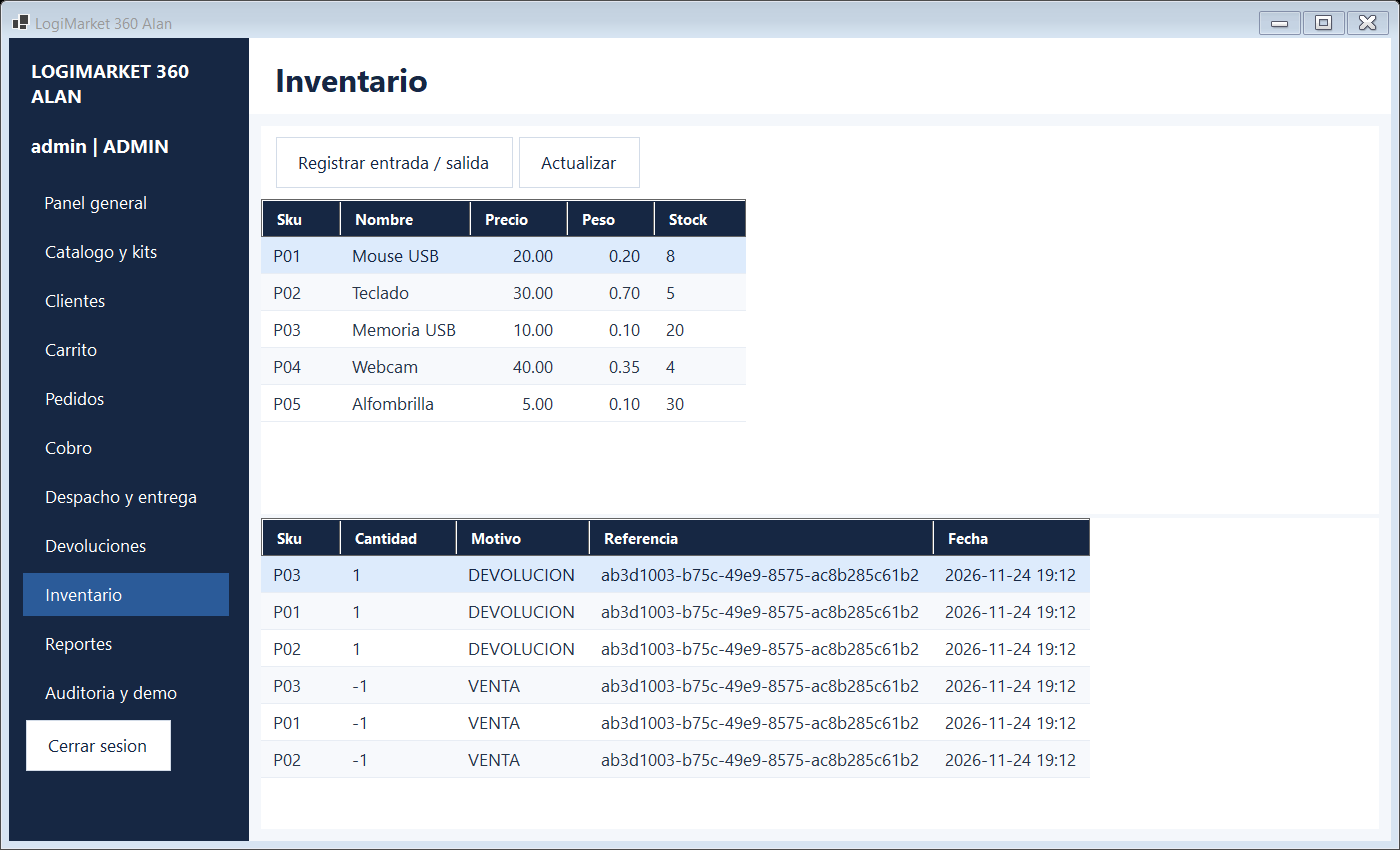
\includegraphics[width=\linewidth,height=9.5cm,keepaspectratio,trim=148.81bp 0.00bp 0.00bp 0bp,clip]{imagenes/flujo-04-reintegro.png}
\captionof{figure}{Inventario después de la devolución aceptada}\label{fig:reintegro}\end{center}
\end{minipage}\par\bigskip
\noindent\begin{minipage}{\linewidth}\subsection{Panel con métricas actualizadas}
El panel muestra un pedido entregado un pago un despacho y una devolución. Las métricas provienen del Singleton y los refrescos se coordinan mediante Mediator.

\begin{center}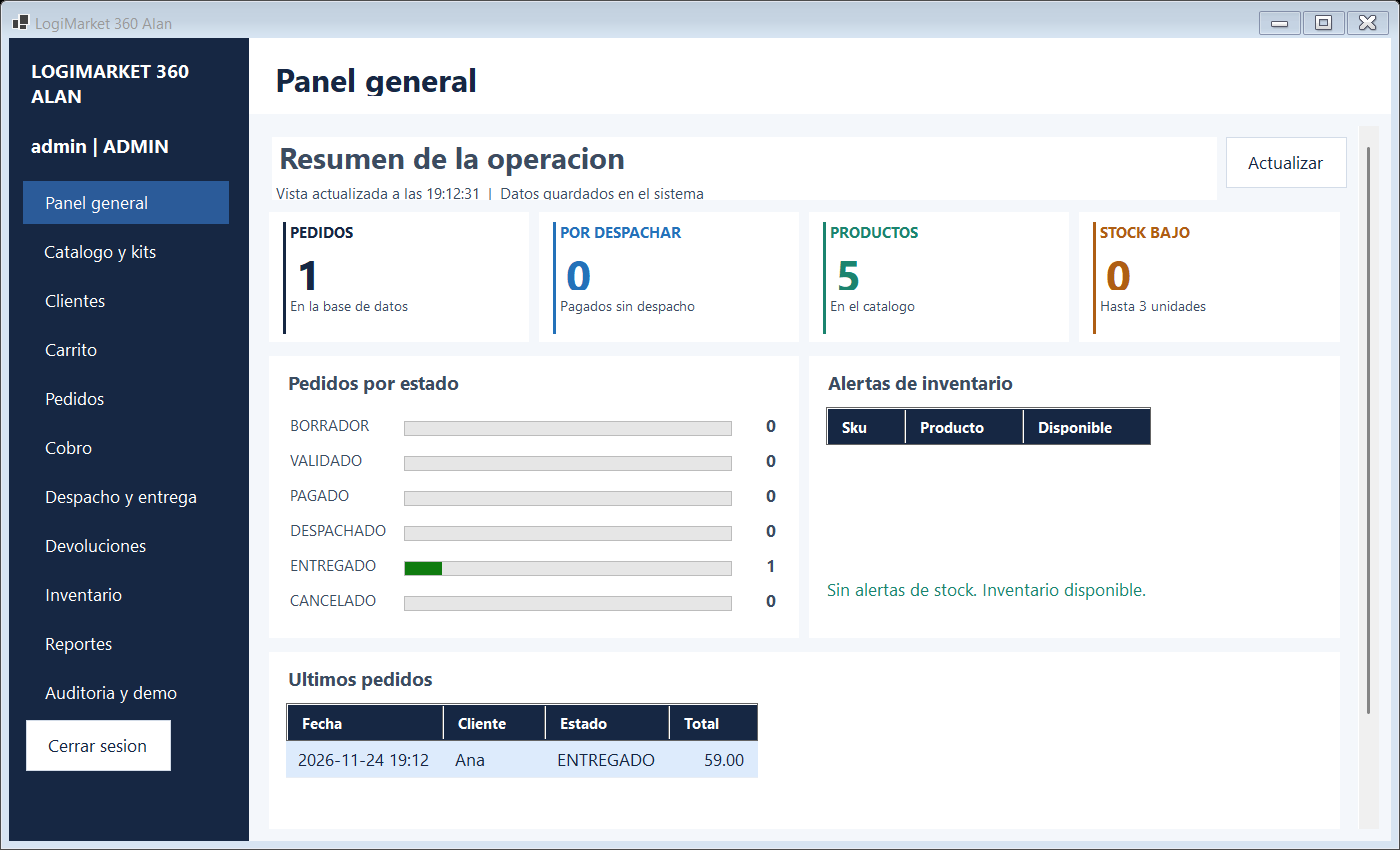
\includegraphics[width=\linewidth,height=9.5cm,keepaspectratio,trim=148.81bp 0.00bp 0.00bp 0bp,clip]{imagenes/flujo-05-metricas.png}
\captionof{figure}{Panel con métricas actualizadas}\label{fig:panel}\end{center}
\end{minipage}\par\bigskip
\noindent\begin{minipage}{\linewidth}\subsection{Comprobante de venta en vista previa}
La ventana muestra el contenido real de ComprobanteVenta. También se generó el archivo TXT mediante la otra implementación de salida.

\begin{center}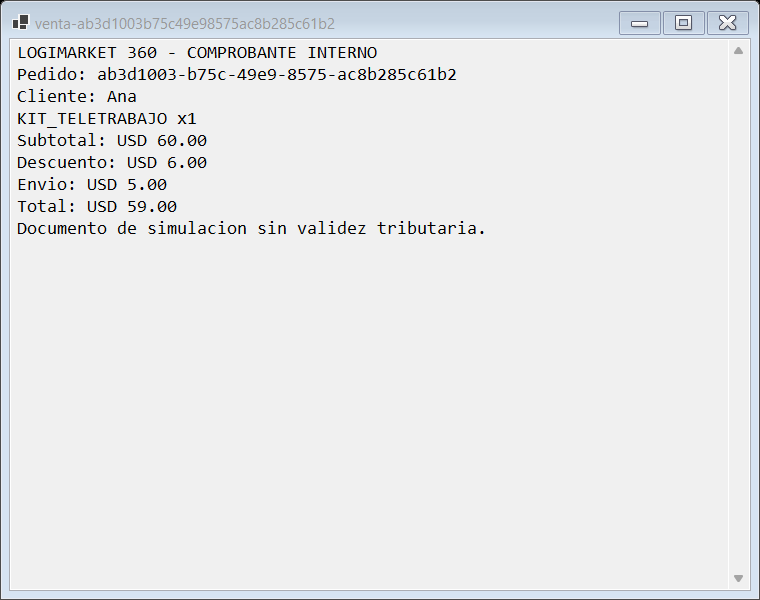
\includegraphics[width=\linewidth,height=9.5cm,keepaspectratio,trim=0.00bp 174.02bp 0.00bp 0bp,clip]{imagenes/bridge-venta.png}
\captionof{figure}{Comprobante de venta en vista previa}\label{fig:bridge-venta}\end{center}
\end{minipage}\par\bigskip
\noindent\begin{minipage}{\linewidth}\subsection{Comprobante de devolución en vista previa}
El documento conserva motivo importe y referencia del reembolso. La salida confirma que no se incluye la tarifa de envío.

\begin{center}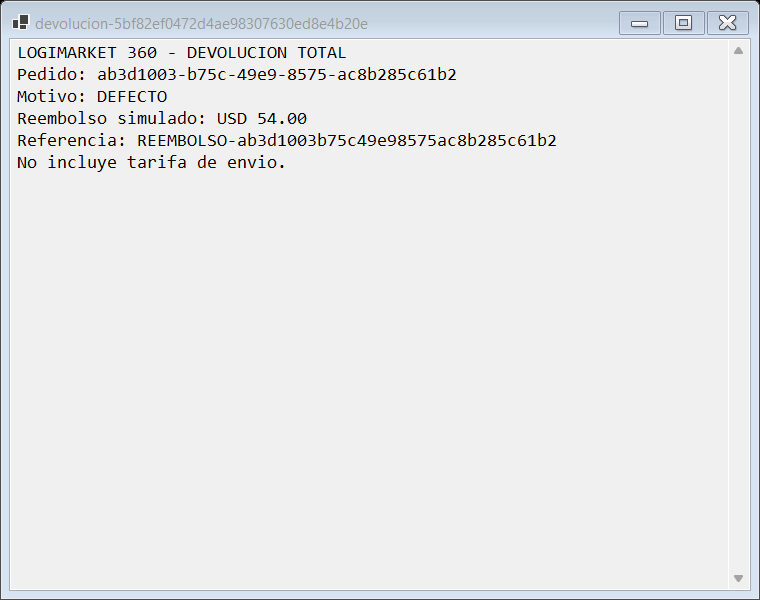
\includegraphics[width=\linewidth,height=9.5cm,keepaspectratio,trim=0.00bp 174.02bp 0.00bp 0bp,clip]{imagenes/bridge-devolucion.png}
\captionof{figure}{Comprobante de devolución en vista previa}\label{fig:bridge-devolucion}\end{center}
\end{minipage}\par\bigskip
\noindent\begin{minipage}{\linewidth}\subsection{Reporte con filtros y salidas de comprobantes}
Interpreter analiza filtros de estado cliente y total Bridge permite elegir venta o devolución y vista previa o TXT La captura corresponde al listado inicial.

\begin{center}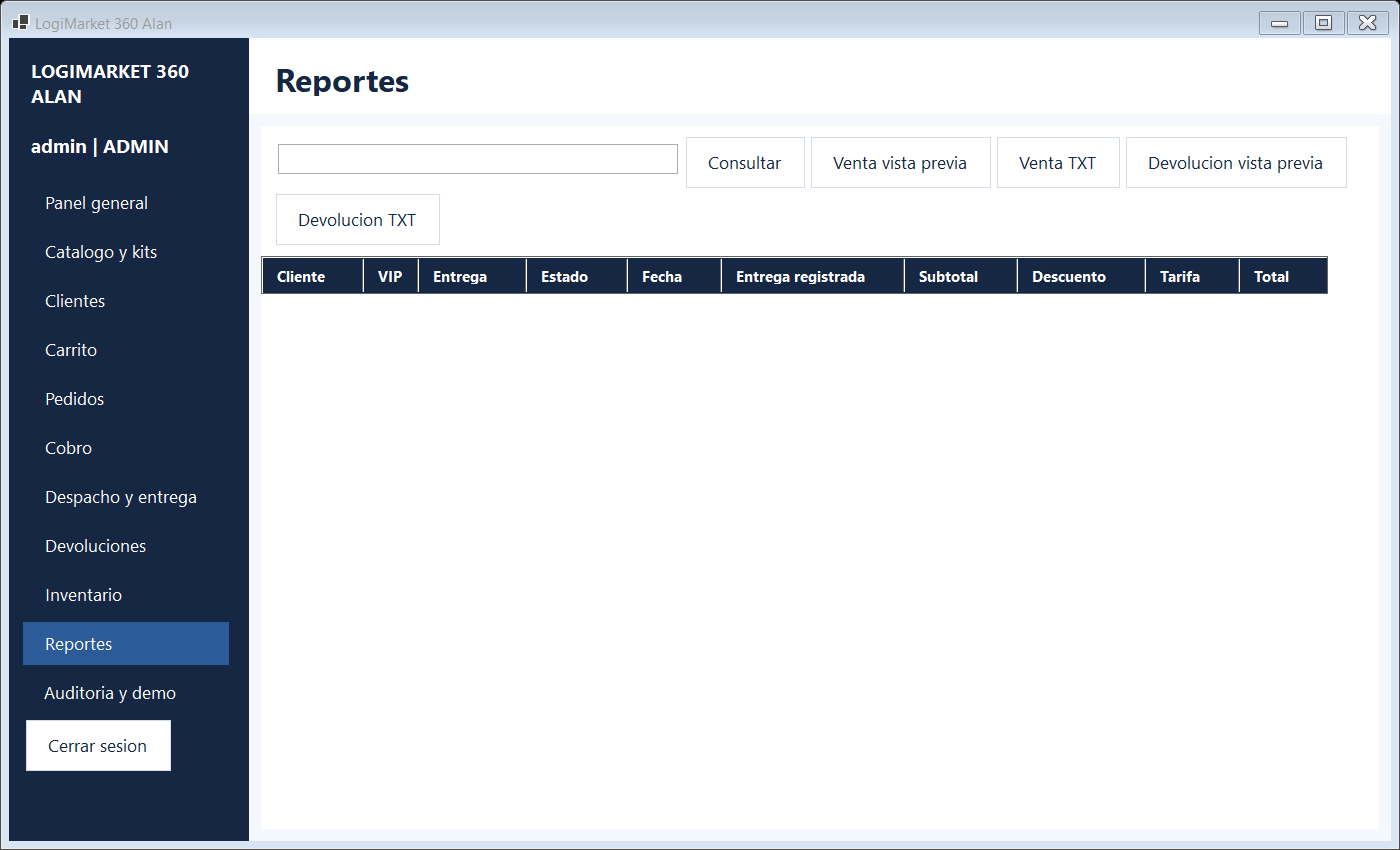
\includegraphics[width=\linewidth,height=9.5cm,keepaspectratio,trim=148.81bp 258.02bp 0.00bp 0bp,clip]{imagenes/vista-Reportes.png}
\captionof{figure}{Reporte con filtros y salidas de comprobantes}\label{fig:reportes}\end{center}
\end{minipage}\par\bigskip
\noindent\begin{minipage}{\linewidth}\subsection{Auditoría y opciones de demostración}
ADMIN puede cambiar proveedor y canal inducir rechazo de cobro o fallo de aviso recuperar Outbox y demostrar Flyweight. Los avisos son locales.

\begin{center}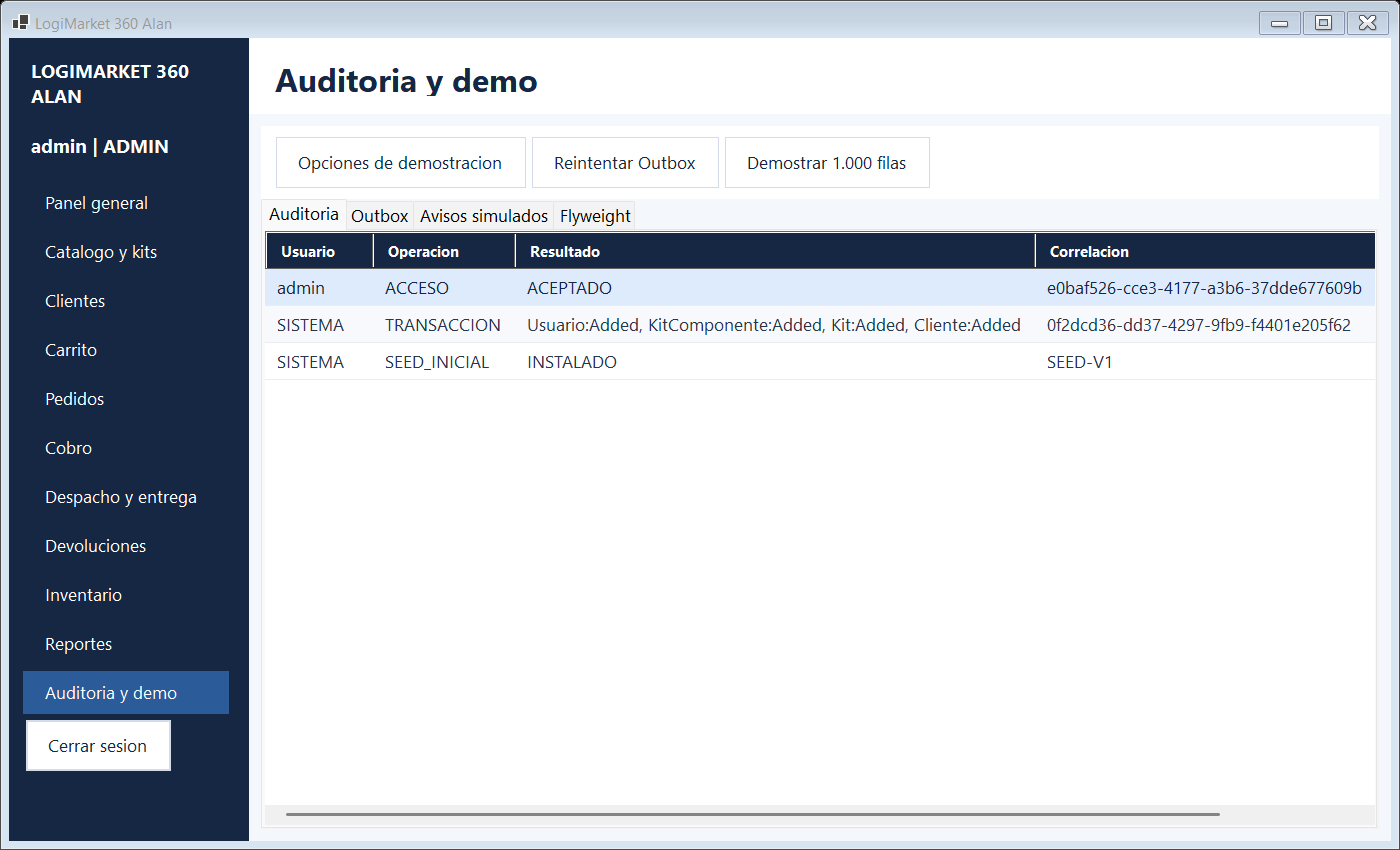
\includegraphics[width=\linewidth,height=9.5cm,keepaspectratio,trim=148.81bp 258.02bp 0.00bp 0bp,clip]{imagenes/vista-Auditoria-y-demo.png}
\captionof{figure}{Auditoría y opciones de demostración}\label{fig:auditoria}\end{center}
\end{minipage}\par\bigskip
